\documentclass[tikz,border=10pt]{standalone}
\usepackage{tikz}
\usetikzlibrary{shapes.geometric,arrows.meta,positioning,calc,decorations.pathmorphing}

\begin{document}
	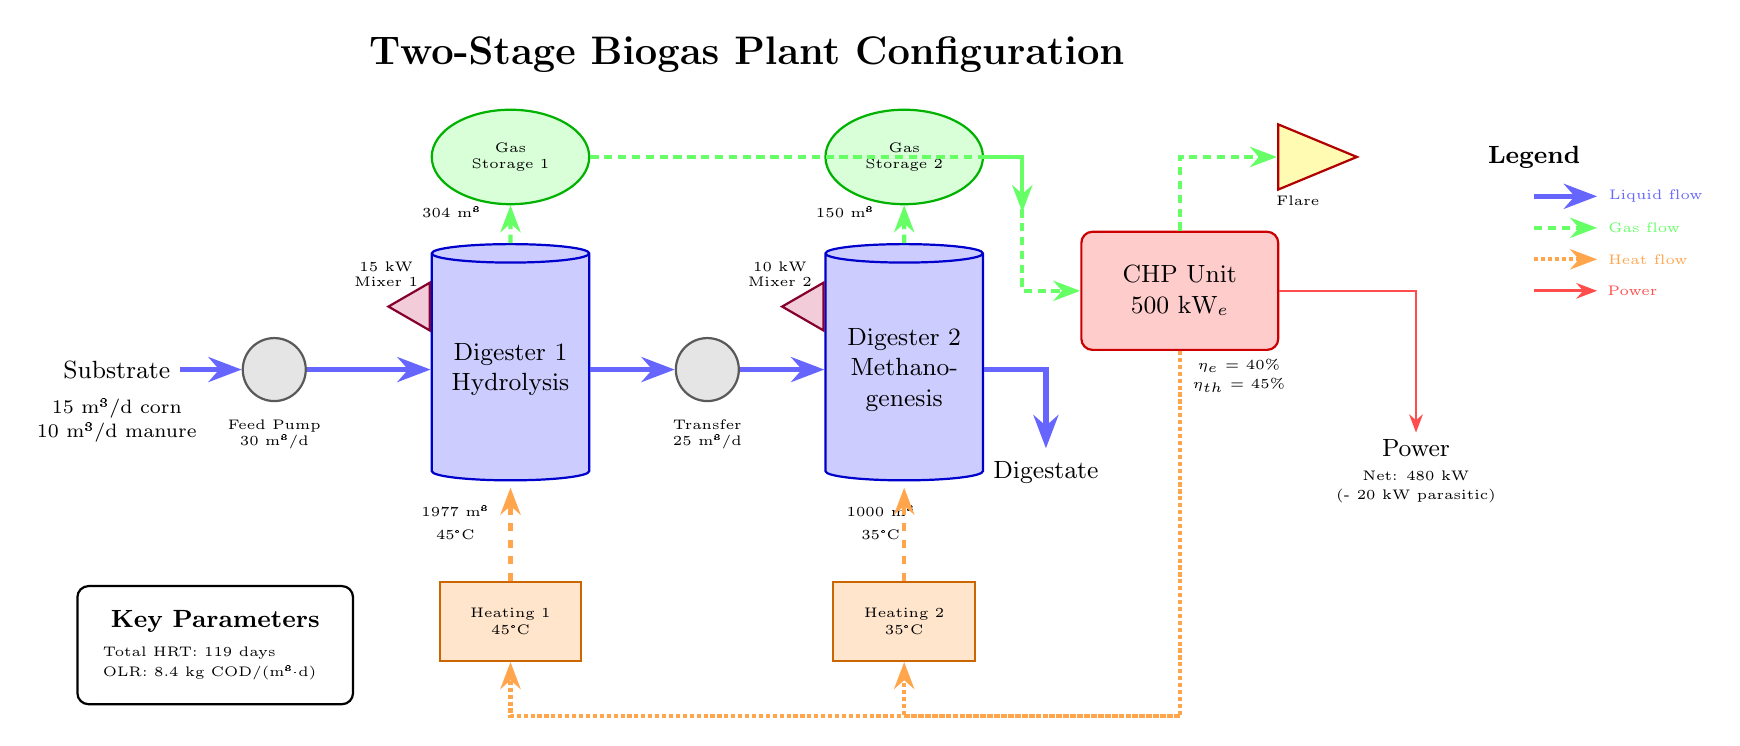
\begin{tikzpicture}[
		% Styles
		digester/.style={cylinder, shape border rotate=90, draw=blue!80!black, fill=blue!20, minimum height=3cm, minimum width=2cm, thick},
		storage/.style={ellipse, draw=green!70!black, fill=green!15, minimum width=2cm, minimum height=1.2cm, thick},
		chp/.style={rectangle, draw=red!80!black, fill=red!20, minimum width=2.5cm, minimum height=1.5cm, thick, rounded corners},
		heating/.style={rectangle, draw=orange!80!black, fill=orange!20, minimum width=1.8cm, minimum height=1cm, thick},
		pump/.style={circle, draw=gray!70!black, fill=gray!20, minimum size=0.8cm, thick},
		mixer/.style={regular polygon, regular polygon sides=3, draw=purple!70!black, fill=purple!20, minimum size=0.7cm, thick},
		flare/.style={isosceles triangle, draw=red!70!black, fill=yellow!30, minimum width=0.8cm, minimum height=1cm, thick},
		% Arrows
		liquid/.style={-Stealth, line width=2pt, blue!60},
		gas/.style={-Stealth, line width=1.5pt, green!60, densely dashed},
		heat/.style={-Stealth, line width=1.5pt, orange!70, densely dotted},
		power/.style={-Stealth, line width=1pt, red!70},
		]

		% Title
		\node[font=\Large\bfseries] at (2,8) {Two-Stage Biogas Plant Configuration};

		% Substrate input
		\node[font=\small] (substrate) at (-6,4) {Substrate};
		\node[font=\scriptsize] at (-6,3.5) {15 m³/d corn};
		\node[font=\scriptsize] at (-6,3.2) {10 m³/d manure};

		% Feed pump
		\node[pump] (feed_pump) at (-4,4) {};
		\node[font=\tiny, below=0.1cm of feed_pump] {Feed Pump};
		\node[font=\tiny, below=0.3cm of feed_pump] {30 m³/d};

		% Digester 1 (Hydrolysis)
		\node[digester] (dig1) at (-1,4) {};
		\node[font=\small, text width=1.8cm, align=center] at (-1,4) {Digester 1\\Hydrolysis};
		\node[font=\tiny] at (-1.7,2.2) {1977 m³};
		\node[font=\tiny] at (-1.7,1.9) {45°C};

		% Mixer 1
		\node[mixer, rotate=90] (mixer1) at (-2.2,4.8) {};
		\node[font=\tiny, above=0.125cm of mixer1] {Mixer 1};
		\node[font=\tiny, above=0.325cm of mixer1] {15 kW};

		% Gas storage 1
		\node[storage] (storage1) at (-1,6.7) {};
		\node[font=\tiny, text width=1.5cm, align=center] at (-1,6.7) {Gas\\Storage 1};
		\node[font=\tiny] at (-1.75,6.0) {304 m³};

		% Transfer pump
		\node[pump] (transfer_pump) at (1.5,4) {};
		\node[font=\tiny, below=0.1cm of transfer_pump] {Transfer};
		\node[font=\tiny, below=0.3cm of transfer_pump] {25 m³/d};

		% Digester 2 (Methanogenesis)
		\node[digester] (dig2) at (4,4) {};
		\node[font=\small, text width=2cm, align=center] at (4,4) {Digester 2\\Methano-\\genesis};
		\node[font=\tiny] at (3.7,2.2) {1000 m³};
		\node[font=\tiny] at (3.7,1.9) {35°C};

		% Mixer 2
		\node[mixer, rotate=90] (mixer2) at (2.8,4.8) {};
		\node[font=\tiny, above=0.125cm of mixer2] {Mixer 2};
		\node[font=\tiny, above=0.325cm of mixer2] {10 kW};

		% Gas storage 2
		\node[storage] (storage2) at (4,6.7) {};
		\node[font=\tiny, text width=1.5cm, align=center] at (4,6.7) {Gas\\Storage 2};
		\node[font=\tiny] at (3.25,6.0) {150 m³};

		% CHP
		\node[chp] (chp) at (7.5,5) {};
		\node[font=\small, text width=2.2cm, align=center] at (7.5,5) {CHP Unit\\500 kW$_e$};
		\node[font=\tiny] at (8.25,4.05) {$\eta_e$ = 40\%};
		\node[font=\tiny] at (8.25,3.8) {$\eta_{th}$ = 45\%};

		% Flare
		\node[flare] (flare) at (9.0,6.7) {};
		\node[font=\tiny, below=0.05cm of flare] {Flare};

		% Heating systems
		\node[heating] (heat1) at (-1,0.8) {};
		\node[font=\tiny, text width=1.6cm, align=center] at (-1,0.8) {Heating 1\\45°C};

		\node[heating] (heat2) at (4,0.8) {};
		\node[font=\tiny, text width=1.6cm, align=center] at (4,0.8) {Heating 2\\35°C};

		% Power output
		\node[font=\small, align=left] at (10.5,3) {Power};
		\node[font=\tiny, align=left] at (10.5,2.65) {Net: 480 kW};
		\node[font=\tiny, align=left] at (10.5,2.4) {(- 20 kW parasitic)};

		% Effluent
		\node[font=\small] at (5.8,2.7) {Digestate};

		% Connections
		% Substrate → Feed pump → Digester 1
		\draw[liquid] (substrate) -- (feed_pump);
		\draw[liquid] (feed_pump) -- (dig1);

		% Digester 1 → Transfer pump → Digester 2
		\draw[liquid] (dig1) -- (transfer_pump);
		\draw[liquid] (transfer_pump) -- (dig2);

		% Gas flows
		\draw[gas] (dig1) -- (storage1);
		\draw[gas] (storage1) -| (5.5,6) |- (chp);
		\draw[gas] (dig2) -- (storage2);
		\draw[gas] (storage2) -| (5.5,6);
		\draw[gas] (chp.north) |- (flare);

		% Heat flows
		\draw[heat] (chp) -- (7.5,-0.4) -| (heat1);
		\draw[heat] (7.5,-0.4) -| (heat2);
		\draw[heat, dashed] (heat1) -- (-1,2.5);
		\draw[heat, dashed] (heat2) -- (4,2.5);

		% Power output
		\draw[power, thick] (chp) -- (10.5,5) -- (10.5,3.2);

		% Effluent
		\draw[liquid] (dig2.east) -| (5.8,3);

		% Legend
		\begin{scope}[shift={(12,6.2)}]
			\node[font=\small\bfseries] at (0,0.5) {Legend};
			\draw[liquid] (0,0) -- (0.8,0) node[right, font=\tiny] {Liquid flow};
			\draw[gas] (0,-0.4) -- (0.8,-0.4) node[right, font=\tiny] {Gas flow};
			\draw[heat] (0,-0.8) -- (0.8,-0.8) node[right, font=\tiny] {Heat flow};
			\draw[power] (0,-1.2) -- (0.8,-1.2) node[right, font=\tiny] {Power};
		\end{scope}

		% Process parameters box
		\draw[rounded corners, thick] (-6.5,1.25) rectangle (-3,-0.25);
		\node[font=\small\bfseries] at (-4.75,0.8) {Key Parameters};
		\node[font=\tiny, align=left, anchor=west] at (-6.3,0.4) {Total HRT: 119 days};
		\node[font=\tiny, align=left, anchor=west] at (-6.3,0.15) {OLR: 8.4 kg COD/(m³·d)};

	\end{tikzpicture}
\end{document}
